\subsection{Understandability}

{
\setbeamertemplate{background canvas}{\tikz[remember picture]\node[opacity=0.45] at (current page.center) {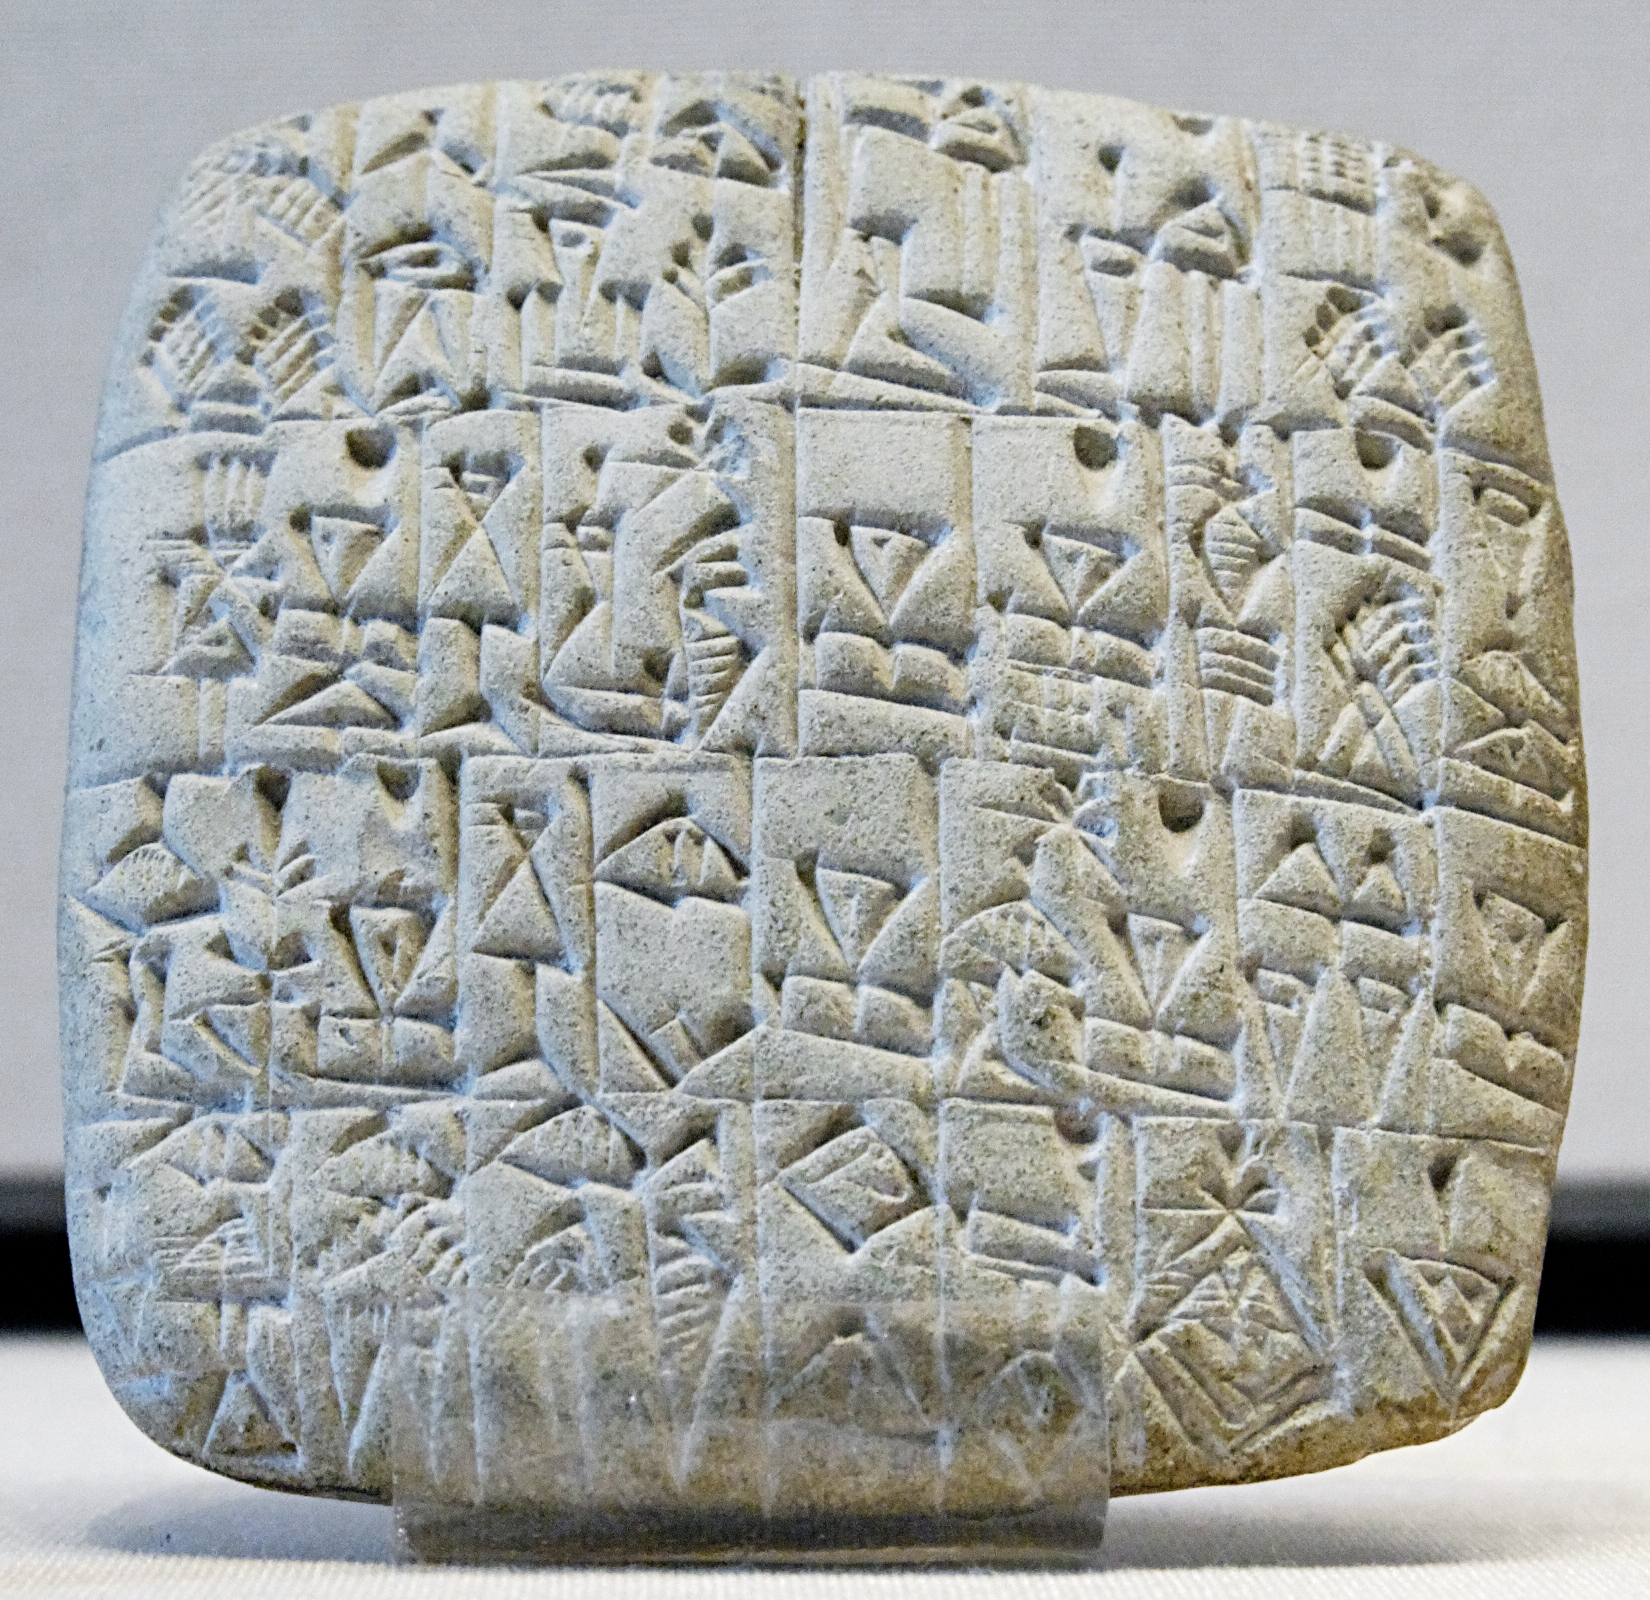
\includegraphics[width=1.155\textwidth,keepaspectratio]{nontex/illustrations/literacy.jpg}};}
\begin{frame}
\frametitle{What Representations Are More Understandable?}
\begin{block}{\begin{large}Knowledge Of Regex Understandability Is Missing\end{large}}
\begin{itemize}
\item \begin{large}understandability is a major pain point\end{large}
\item \begin{large}comprehension tests can determine understandability\end{large}
\end{itemize}
\end{block}
\end{frame}
}
\note[itemize]{
    \item https://upload.wikimedia.org/wikipedia/commons/5/58/Bill_of_sale_Louvre_AO3765.jpg
}

%------------------------------------------------

\begin{frame}[fragile]
\frametitle{Covering Edges}
\begin{center}
14 edges covered by 35 regex pairs
\\*Matching challenge for each regex given to 30 participants
\end{center}
\begin{columns}[t]
\column{.5\textwidth}
\begin{figure}
  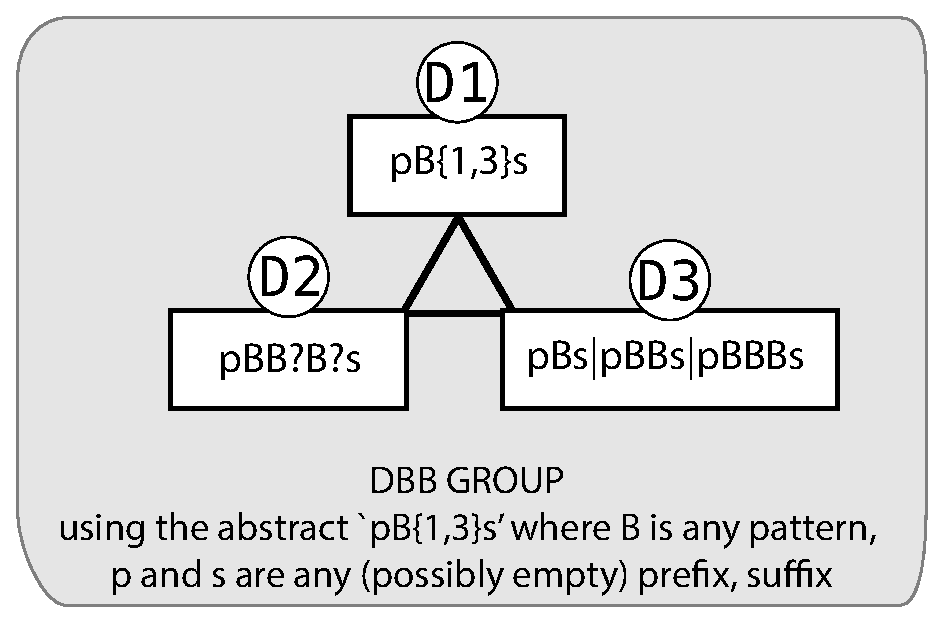
\includegraphics[scale=0.35]{nontex/illustrations/DBBExample.eps}
  \label{fig:DBBExample}
\end{figure}
\column{.5\textwidth}
\begin{itemize}
\item[D1] \cverb!((q4f){0,1}ab)!
\item[D2] \cverb!((q4f)?ab)!
\item[D3] \cverb!(q4fab|ab)!
\item[TRUE] \verb|"ab"|
\item[FALSE] \verb|"fq4f"|
\item[TRUE] \verb|"xyzq4fab"|
\item[TRUE] \verb|"zlmab"|
\item[FALSE] \verb|"qfa4"|
\end{itemize}
\end{columns}
\end{frame}
\note[itemize]{
    \item pt 1
    \item pt 2
}

%------------------------------------------------

\begin{frame}
\frametitle{Testing Comprehension}
% \begin{columns}[t]
% \column{.5\textwidth}
% \begin{figure}
%   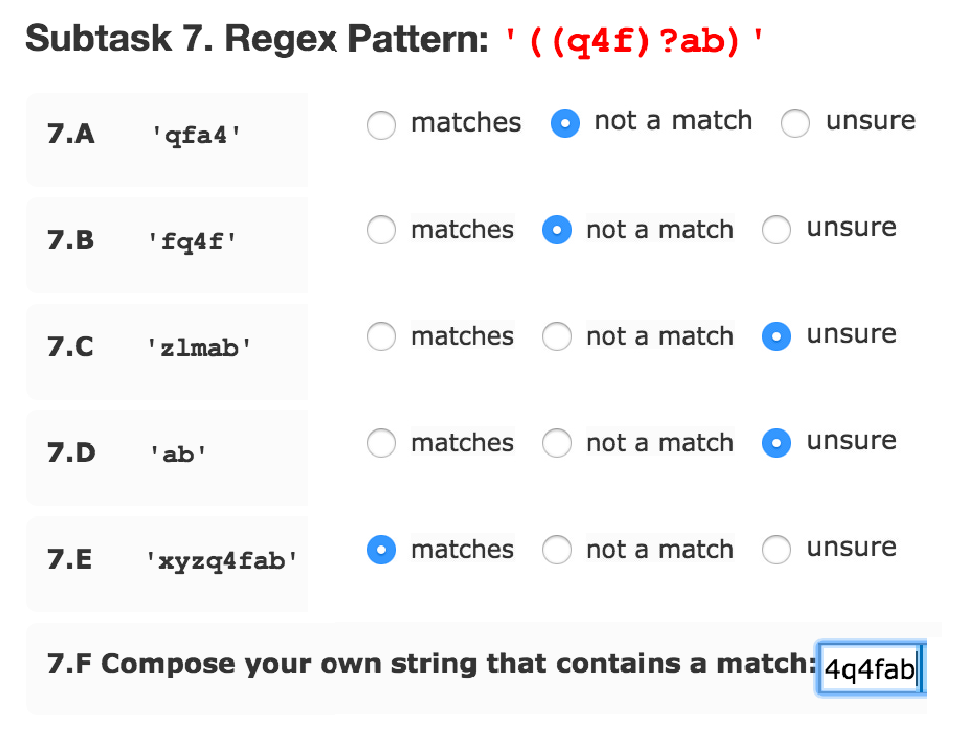
\includegraphics[scale=0.35]{nontex/illustrations/exampleQuestion.eps}
%   \label{fig:exampleQuestion}
% \end{figure}
% \column{.5\textwidth}
% \input{table/matchingMetric}
% \end{columns}
\begin{center}
180 participants answered one composition and five string matching questions for 10 regexes: 10,800 data points total.
\end{center}
\begin{figure}
  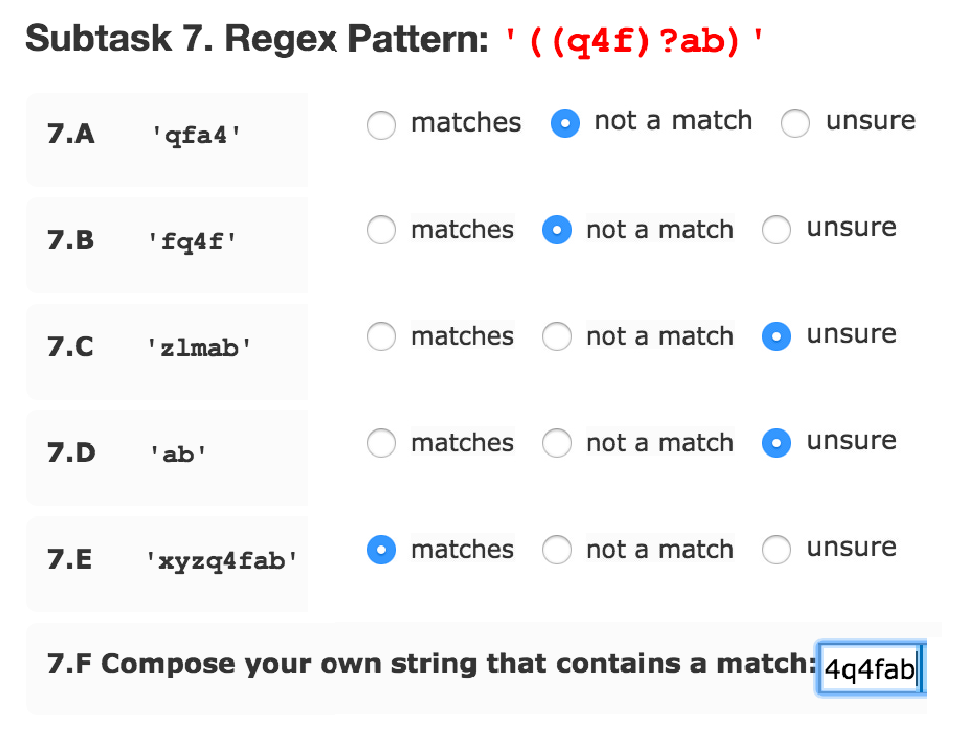
\includegraphics[scale=0.48]{nontex/illustrations/exampleQuestion.eps}
  \label{fig:exampleQuestion}
\end{figure}
\end{frame}
\note[itemize]{
    \item pt 1
    \item pt 2
}

%------------------------------------------------


\begin{frame}
\frametitle{Combined Edge Info}
\begin{adjustbox}{width=\textwidth}\begin{tabular}
{llccccccc}
\textbf{Index} & \textbf{Nodes} & \textbf{Pairs} & \textbf{Match1} & \textbf{Match2} & \textbf{$H_0^{match} $} & \textbf{Compose1} & \textbf{Compose2} &  \textbf{$H_0^{comp}$}  \\
\toprule[0.16em]
E1 & T1 -- T4 & 2 & 80\% & 60\% & 0.001 & 87\% & 37\% & $<$\textbf{0.001}\\
E2 & D2 -- D3 & 2 & 78\% & 87\% & \textbf{0.011} & 88\% & 97\% & 0.085\\
E3 & C2 -- C5 & 4 & 85\% & 86\% & 0.602 & 88\% & 95\% & \textbf{0.063}\\
E4 & C2 -- C4 & 1 & 83\% & 92\% & \textbf{0.075} & 60\% & 67\% & 0.601\\
\midrule[0.05em]
E5 & L2 -- L3 & 2 & 86\% & 91\% & 0.118 & 97\% & 100\% & 0.159\\
E6 & D1 -- D2 & 2 & 84\% & 78\% & 0.120 & 93\% & 88\% & 0.347\\
E7 & C1 -- C2 & 2 & 94\% & 90\% & 0.121 & 93\% & 90\% & 0.514\\
E8 & T2 -- T4 & 2 & 84\% & 81\% & 0.498 & 65\% & 52\% & 0.141\\
E9 & C1 -- C5 & 2 & 94\% & 90\% & 0.287 & 93\% & 93\% & 1.000\\
E10 & T1 -- T3 & 3 & 88\% & 86\% & 0.320 & 72\% & 76\% & 0.613\\
E11 & D1 -- D3 & 2 & 84\% & 87\% & 0.349 & 93\% & 97\% & 0.408\\
E12 & C1 -- C4 & 6 & 87\% & 84\% & 0.352 & 86\% & 83\% & 0.465\\
E13 & C3 -- C4 & 2 & 61\% & 67\% & 0.593 & 75\% & 82\% & 0.379\\
E14 & S1 -- S2 & 3 & 85\% & 86\% & 0.776 & 88\% & 90\% & 0.638\\
\bottomrule[0.13em]\end{tabular}
\end{adjustbox}

\end{frame}
\note[itemize]{
    \item pt 1
    \item pt 2
}

%------------------------------------------------



\begin{frame}
\frametitle{Four Significant Understandability Differences, $\alpha=0.1$}
\begin{adjustbox}{width=\textwidth}
\begin{tabular}
{lccc c lccc}
\textbf{Code} & \textbf{Regex} & \textbf{Match} & \textbf{Compose} & \textbf{Refactoring} & \textbf{Node} & \textbf{Regex} & \textbf{Match} & \textbf{Compose}  \\
\noalign{\hrule height 0.08em}
T4 & \begin{minipage}{0.9in}\cverb!([\072\073])!\end{minipage} & 66\% & 50\% & $\overrightarrow{T4 T1}$ & T1 & \begin{minipage}{1.2in}\cverb!([:;])!\end{minipage} & 81\% & 87\%    \\
T4 & \begin{minipage}{0.9in}\cverb!([\0175\0173])!\end{minipage} & 54\% & 23\% & & T1 & \begin{minipage}{1.2in}\cverb!([}{])!\end{minipage} & 79\% & 87\%     \\
\noalign{\hrule height 0.04em}
D2 & \begin{minipage}{0.9in}\cverb!((q4f)?ab)!\end{minipage} & 79\% & 83\% & $\overrightarrow{D2 D3}$ & D3 & \begin{minipage}{1.2in}\cverb!(q4fab|ab)!\end{minipage} & 85\% & 97\%     \\
D2 & \begin{minipage}{0.9in}\cverb!(deedo(do)?)!\end{minipage} & 77\% & 93\% & & D3 & \begin{minipage}{1.2in}\cverb!(deedo|deedodo)!\end{minipage} & 90\% & 97\%     \\
\noalign{\hrule height 0.08em}
C2 & \begin{minipage}{0.9in}\cverb!([:;])!\end{minipage} & 81\% & 87\% & $\overrightarrow{C2 C5}$ & C5 & \begin{minipage}{1.2in}\cverb!(:|;)!\end{minipage} & 94\% & 100\%     \\
C2 & \begin{minipage}{0.9in}\cverb!no[wxyz]5!\end{minipage} & 87\% & 90\% &  & C5 & \begin{minipage}{1.2in}\cverb!no(w|x|y|z)5!\end{minipage} & 94\% & 97\%     \\
C2 & \begin{minipage}{0.9in}\cverb!([}{])!\end{minipage} & 79\% & 87\% & & C5 & \begin{minipage}{1.2in}\cverb!(\{|\})!\end{minipage} & 70\%  & 93\%    \\
C2 & \begin{minipage}{0.9in}\cverb!tri[abcdef]3!\end{minipage} & 93\% & 90\% & & C5 & \begin{minipage}{1.2in}\cverb!tri(a|b|c|d|e|f)3!\end{minipage} & 86\% & 90\%     \\
\noalign{\hrule height 0.04em}
C2 & \begin{minipage}{0.9in}\cverb![\t\r\f\n ]!\end{minipage} & 83\% & 60\% & $\overrightarrow{C2 C4}$ & C4 & \begin{minipage}{1.2in}\cverb![\s]!\end{minipage} & 92\%  & 67\%    \\
\noalign{\hrule height 0.08em}
\end{tabular}
\end{adjustbox}

\end{frame}
\note[itemize]{
    \item pt 1
    \item pt 2
}

%------------------------------------------------

\begin{frame}
\frametitle{Four Noteworthy Trends}
\begin{table}[!ht]
\begin{center}
\caption{Additional equivalent regexes for which some preference in understandability is suggested}
\label{table:interestingEdges}
\begin{small}
\begin{tabular}
{lccc c lccc}
\textbf{Node} & \textbf{Regex} & \textbf{Match} & \textbf{Compose} & \textbf{Ref.} & \textbf{Node} & \textbf{Regex} & \textbf{Match} & \textbf{Compose} \bigstrut \\
\noalign{\hrule height 0.08em}
L2 & \begin{minipage}{0.92in}\cverb!zaa*!\end{minipage} & 87\% & 97\% & \multirow{ 2}{*}{$\overrightarrow{L2 L3}$} & L3 & \begin{minipage}{1.0in}\cverb!za+!\end{minipage} & 91\% & 100\%  \bigstrut   \\
L2 & \begin{minipage}{0.92in}\cverb!RR*!\end{minipage} & 86\% & 97\% & & L3 & \begin{minipage}{1.0in}\cverb!R+!\end{minipage} & 92\%  & 100\%  \bigstrut  \\
\noalign{\hrule height 0.04em}
D2 & \begin{minipage}{0.92in}\cverb!((q4f)?ab)!\end{minipage} & 79\% & 83\% & \multirow{ 2}{*}{$\overrightarrow{D2 D1}$} & D1 & \begin{minipage}{1.0in}\cverb!((q4f){0,1}ab)!\end{minipage} & 83\% & 97\%  \bigstrut   \\
D2 & \begin{minipage}{0.92in}\cverb!(deedo(do)?)!\end{minipage} & 77\% & 93\% &  & D1 & \begin{minipage}{1.0in}\cverb!(dee(do){1,2})!\end{minipage} & 85\% & 90\%  \bigstrut   \\
\noalign{\hrule height 0.04em}
C2 & \begin{minipage}{0.92in}\cverb!tri[abcdef]3!\end{minipage} & 93\% & 90\% & \multirow{ 2}{*}{$\overrightarrow{C2 C1}$} & C1 & \begin{minipage}{1.0in}\cverb!tri[a-f]3!\end{minipage} & 94\% & 97\%  \bigstrut   \\
C2 & \begin{minipage}{0.92in}\cverb!no[wxyz]5!\end{minipage} & 87\% & 90\% & & C1 & \begin{minipage}{1.0in}\cverb!no[w-z]5!\end{minipage} & 93\%  & 90\%  \bigstrut  \\
\noalign{\hrule height 0.08em}
T4 & \begin{minipage}{0.92in}\begin{footnotesize}\cverb!xyz[\0133-\0140]!\end{footnotesize}\end{minipage} & 71\% & 33\% & \multirow{ 2}{*}{$\overrightarrow{T4 T2}$} & T2 & \begin{minipage}{1.0in}\cverb!xyz[\x5b-\x5f]!\end{minipage} & 79\% & 60\%  \bigstrut   \\
T4 & \begin{minipage}{0.92in}\cverb!t[\072-\073]+p!\end{minipage} & 90\% & 70\% &  & T2 & \begin{minipage}{1.0in}\cverb!t[\x3a-\x3b]+p!\end{minipage} & 89\% & 70\%  \bigstrut   \\
\noalign{\hrule height 0.08em}
\end{tabular}
\end{small}
\end{center}
\vspace{-12pt}
\end{table}

\end{frame}
\note[itemize]{
    \item pt 1
    \item pt 2
}

%------------------------------------------------
